\chapter{Bitcoin: moneta elettronica decentralizzata}\label{bitcoin-moneta-elettronica-decentralizzata}

Tutte le reti P2P finora descritte sono in circolazione da molti anni, hanno una base di utenti che conta milioni di peer divisi tra utenti reali e server automatizzati, contano migliaia di forum di supporto e scambiano quotidianamente una immensa fetta del traffico totale della rete Internet (tanto che molti provider tendono a limitarne quanto più possibile l'utilizzo, soprattutto nelle fasce orarie di maggior traffico). Sono però tutte reti dedicate al file-sharing. Bitcoin no. O almeno, non proprio, come vedremo.

Bitcoin è una rete P2P (intesa per tutti e tre i livelli descritti in precedenza) che mira a creare un sistema di valuta digitale privo di controllo centrale, con pagamenti effettuati direttamente tra gli utenti senza l'intervento di terzi. È stata ideata e realizzata in origine da un anonimo noto con il nome di \textbf{Satoshi Nakamoto} \cite{bitcoin}, formalizzata con un whitepaper nel 2008 ed entrata in vigore il 3 Gennaio 2009 e si è in poco tempo evoluta in modo esponenziale fino a catturare di recente l'attenzione dei media internazionali, delle banche mondiali e, per alcuni suoi utilizzi illeciti, da FBI ed NSA. Ma vediamo di cosa si tratta.

\section{Moneta Elettronica}\label{moneta-elettronica}

\textbf{Bitcoin} è il nome dato alla rete, al client originale, al protocollo di comunicazione e alla moneta utilizzata per le transazioni all'interno della rete.

Le monete (d'ora in avanti \textbf{btc}) posso essere ottenute ``gratuitamente'' dopo aver impegnato la propria CPU o GPU in alcuni calcoli di crittografia (operazione chiamata \textbf{mining} e discussa più avanti), oppure acquistate da altri utenti della rete tramite una valuta reale \footnote{Ad esempio tramite il sito Internet Mt. Gox   \cite{mtgox}.}.

Entrambi questi metodi sono fondamentali nell'ecosistema Bitcoin:

\begin{itemize}
\item
  Il mining è una diretta conseguenza della partecipazione di un nodo   alla rete (vedi più avanti NETWORK) ed è l'unico metodo con cui   vengono create e messe in circolazioni nuove \textbf{btc}. Per ogni   operazione di mining avvenuta con successo si riceve una quantità   fissa di btc che viene dimezzata nel tempo, limitando il numero   massimo di bitcoin in circolazione a circa 21 milioni. A Gennaio 2013   è stata generata circa la metà delle monete totali e si stima di   arrivare a 3/4 nel 2017. La quota massima di moneta circolante e   l'assenza di istituti centrali in grado di creare nuove monete rendono   l'economia bitcoin invulnerabile all'inflazione che colpisce le   economie reali. Il sistema è ispirato a quella che era l'economia del   Dollaro prima della istituzionalizzazione della Federal Reserve come   banca federale: il valore del Dollaro era legato al valore corrente   dell'oro, il quale esiste in quantità limitata ed è ottenibile solo   attraverso il lavoro dei minatori.
\item
  La compravendita di bitcoin è invece simile alle compravendite di   azioni effettuate nelle borse di tutte il mondo. Esistono infatti   alcuni luoghi dedicati (ad esempio il sito internet \emph{Mt. GOX})   che fungono da stock exchange offrendo agli utenti la possibilità di   mettere in vendita o di acquistare bitcoin al prezzo che preferiscono.   Sono delle vere e proprie borse che trattano unicamente bitcoin invece   che molti titoli di aziende diverse, calcolano un valore di scambio   medio basato sulle ultime transazioni portate a termine ma lasciano   libero l'utente di scegliere a quanto vendere o comprare bitcoin, con   prezzo medio che si adegua di conseguenza. 
%FIXME sistemare sta roba   
%TODO verificare se rapporto bitcoin/euro e bitcoin/dollaro sono   legati alle transazioni in quella valuta (come credo che sia)
\end{itemize}

Come per le monete in valuta reale e le azioni borsistiche, anche le bitcoin vengono ``tenute'' in portafogli. Come vedremo, il termine \emph{tenute} è usato impropriamente, ma questa è l'apparenza dal punto di vista dell'utente, per cui a tale apparenza al momento ci atterremo.

\section{Portafogli e indirizzi}\label{portafogli-e-indirizzi}

La prima volta che un nuovo utente avvia il suo client Bitcoin fresco di installazione, si vede assegnato un portafoglio contenente un indirizzo e una copia di chiavi di cifratura simmetrica. L'indirizzo è semplicemente una stringa di 27-34 caratteri alfanumerici che inizia con un 1 o con un 3, generata in modo casuale dalle chiavi create per l'utente. Gli indirizzi rappresentano il punto di uscita e/o il punto di ingresso per tutti i movimenti che coinvolgono bitcoin. Questo significa che nelle transazioni bitcoin compariranno unicamente questi indirizzi, rendendo di fatto \textbf{anonimi} tutti i movimenti di bitcoin (meno quelli che riguardano l'acquisto di bitcoin tramite moneta reale), in un modo del tutto equivalente a quello dei conti in Svizzera. Non esiste quindi nessuna correlazione diretta e ovvia tra un utente e il suo indirizzo. Un portafogli può contenere più indirizzi: basta infatti generare una nuova coppia di chiavi e verrà generato anche un nuovo indirizzo. Il numero di indirizzi esistenti è virtualmente infinito.

I portafogli sono solitamente legati al software che li crea, basta quindi cambiare software per poter creare un nuovo portafogli e una nuova coppia di chiavi (oppure installare un software in grado di gestire più portafogli). In alternativa è possibile ``aprire un conto'' presso numeri siti che offrono questa funzionalità, quale ad esempio blockchain.info. In questo caso però bisogna fare i conti con la sicurezza del sito in questione 
%TODO link alla sezione sicurezza

\section{Transazioni}\label{transazioni}

Le transazioni rappresentano il nucleo fondamentale di bitcoin. Esse sono il metodo con cui, a livello astratto, le bitcoin vengono trasferite da un account all'altro e tramite la loro analisi ci si assicura che un indirizzo contenga esattamente quel numero di bitcoin, che una bitcoin non venga spesa più volte e che quella bitcoin appartiene a quello specifico indirizzo. Le transazioni si basano su meccanismi di crittografia a chiave pubblica, rendendo quindi obsoleto il coinvolgimento di terze parti nella transazione. Se infatti nelle normali compravendite online, volenti o nolenti si è costretti a fidarsi di terze parti che garantiscono per il buon esito dell'operazione (istituti di credito, compagnie di carte di credito, siti come Paypal, ecc), qui gli utenti hanno direttamente la prova crittografica senza aver quindi necessita di fidarsi di qualcuno.

Satoshi Nakamoto descrive la sua moneta elettronica come una serie di firme digitali. Il trasferimento di moneta da un utente all'altro avviene infatti applicando la firma digitale dell'acquirente ad un hash di una precedente transazione e della chiave pubblica del venditore, e aggiungendo ciò alla fine della moneta.

Riassumendo schematicamente:

\begin{verbatim}
hash = hash(previous_transaction, vendor_public_key)
transaction = sign(hash, private_key)
\end{verbatim}

La moneta diventa quindi non una unità atomica, ma il risultato di una serie di transazioni che coinvolgono firme digitali e verifiche che deve essere calcolato dinamicamente. La serie di tutte le transazioni mai effettuate viene raccolta in una sequenza denominata \textbf{blockchain}.

\begin{figure}[htbp]
\centering
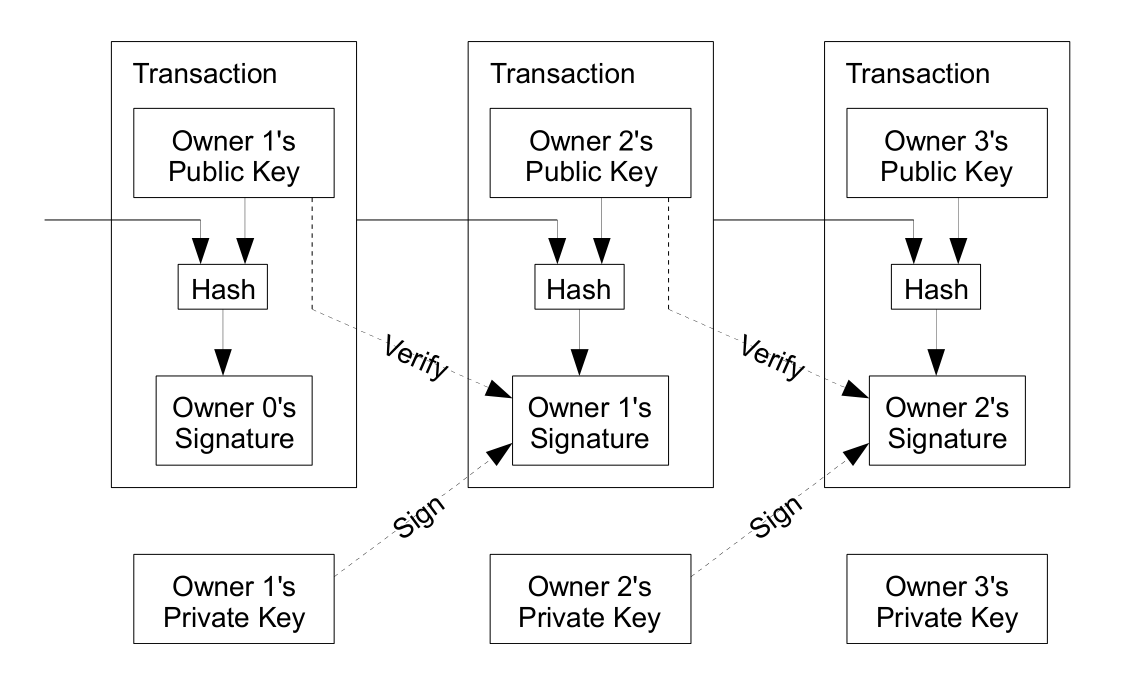
\includegraphics{bitcoin_p2_1.PNG}
\caption{Utilizzo delle chiavi e degli hash in una sequenza di transazioni.\label{bitcoin_p2_1}}
\end{figure}

Questa implementazione però non garantisce che l'acquirente non abbia già effettuato una transazione con questa moneta, ovvero che stia spendendo una moneta già spesa in precedenza.

L'unico modo per garantire ciò senza utilizzare una terza parte di cui fidarsi, è tenere conto di \textbf{tutte} le transazioni. Questo vuol dire che tutte le transazioni devono essere annunciate ad un pubblico in grado di mettersi d'accordo sull'effettivo ordine temporale in cui sono state effettuate. Il venditore deve avere quindi la prova che, nel momento in cui riceve la transazione, la maggioranza dei nodi è d'accordo che quella è la prima transazione ricevuta.i

\section{Timestamp e Proof-of-Work}\label{timestamp-e-proof-of-work}

La soluzione consiste nell'utilizzo di un \textbf{timestamp server}. Un timestamp server funziona calcolando l'hash di un blocco di oggetti di cui si vuole realizzare il timestamp e rendendo tale hash pubblico. Il timestamp dimostra inequivocabilmente che gli oggetti esistevano al momento dell'hashing. Ogni timestamp include anche il precedente timestamp nell'hash, formando quindi una catena in cui ogni timestamp rinforza \footnote{leggasi: rende più difficili da modificare.} quelli precedenti.

Ora il problema consiste nell'implementare questo server di timestamp in modo distribuito, come è appunto la rete Bitcoin. Per prima cosa bisogna trovare un sistema per cui effettuare il timestamp è un'operazione difficoltosa (computazionalmente parlando), ma verificare che il timestamp sia corretto deve essere immediato. Basandosi sul lavoro di Adam Back (\cite{hashcash}), Nakamoto ha deciso che la difficoltà dell'operazione deve essere trovare un valore che, una volta sottoposto ad hashing (ad esempio con SHA-256), il risultato sia un hash che comincia con uno specifico numero di bit pari a zero: la difficoltà del lavoro è esponenziale al numero di bit zero richiesti, ma è facilmente verificabile con un singolo hash. L'implementazione per bitcoin consiste quindi nella creazione di un blocco di dati di cui calcolare l'hash che contiene le transazioni interessate, l'hash precedente e un valore chiamato \textbf{nonce} da incrementare fino a quando l'hash non avrà le caratteristiche richieste. Modificare una transazione comporta modificare un blocco, e quindi ripetere tutto il lavoro di calcolo della nonce. Inoltre, se a questo blocco è già stato incatenato uno più blocchi successivi, anche tali blocchi andranno ricalcolati in sequenza, rendendo il lavoro estremamente gravoso.

\begin{figure}[htbp]
\centering
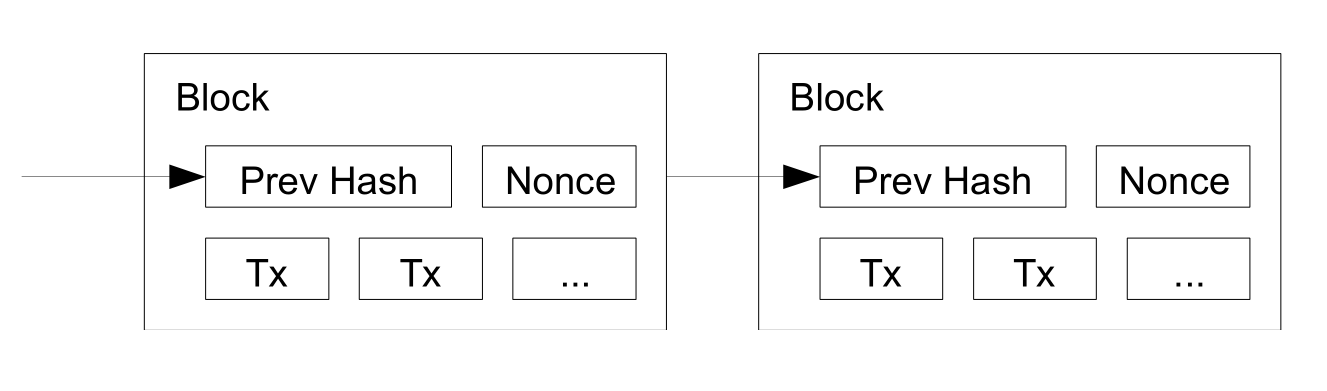
\includegraphics{bitcoin_p3_1.PNG}
\caption{Struttura minimale di una sequenza di blocchi.\label{bitcoin_p3_1}}
\end{figure}

Con la prova di lavoro si risolve anche il problema di cosa significa che la maggioranza deve accettare un timestamp. Con l'hash infatti si realizza una sorta di sistema one-CPU-one-vote, e la ``decisione della maggioranza'' è rappresentata dalla più lunga sequenza di timestamp, che è la sequenza per la quale è stata impiegata la maggior parte di lavoro computazionale. Ciò significa che se la maggior parte della forza-CPU è controllata da peer onesti (cioè che non hanno nessuna intenzione di modificare una transazione effettuata), un nodo disonesto che volesse modificare una transazione non solo dovrebbe rifare tutti i calcoli per il blocco della transazione e per tutti i blocchi successivi, ma avendo minor potenza di CPU a disposizione rispetto ai nodi onesti, verrebbe rapidamente soverchiato dal numero di calcoli da fare, in quando il numero di blocchi da ricalcolare sarebbe sempre superiori a quelli da lui già ricalcolati.

Si capisce subito che è nella rete bitcoin (e nelle reti P2P in generale) è importante che le risorse (potenza di calcolo in questo caso) siano equamente distribuite tra i peer, in modo da evitare che un solo nodo o un solo gruppo di nodi controlli l'intera rete.

Per far fronte alle differenti configurazioni hardware degli utenti, alla sempre crescente capacità di calcolo di CPU e GPU e anche ai potenzialmente mutevoli interessi dei nodi, la difficoltà della prova di lavoro (ovvero il numero di bit zero) è determinata da una media calcolata sul numero medio di blocchi generati ogni ora. Se vengono generati troppi blocchi, vuol dire che la difficoltà è troppo bassa e viene subito aumentata.

\section{Network}\label{network}

A questo punto abbiamo una prima approssimazione di come funziona la rete bitcoin:

\begin{enumerate}
\def\labelenumi{\arabic{enumi}.}
\itemsep1pt\parskip0pt\parsep0pt
\item
  Le nuove transazioni sono inviate a tutti i nodi.
\item
  Ogni nodo raccoglie le transazioni che riceve in un blocco.
\item
  Per ogni blocco, ogni nodo cerca di calcolare una proof-of-work.
\item
  Una volta trovata la prova, invia il blocco a tutti i nodi.
\item
  I nodi accettano il nuovo blocco se e solo se tutte le transazioni in   esso sono valide (si verifica calcolando l'hash delle transazioni e   confrontandole con l'ultimo blocco accettato) e non già spese in   precedenza.
\item
  Il nodo esprime la sua accettazione del blocco appena arrivato   mettendosi al lavoro per crearne uno nuovo, usando l'hash del nodo   accettato.
\end{enumerate}

I nodi considerano la catena più lunga quella corretta (e viene definita \emph{blockchain}) e lavoreranno sempre in modo da prolungarla. Esiste la possibilità che uno stesso nodo riceva due versioni diverse dello stesso blocco in contemporanea. In questo caso, lavoreranno sul prima blocco ricevuto, ma manterrano una copia anche dell'altro nel caso in cui si rivelasse appartenente alla catena più lunga. La verifica viene fatta non appena viene trovata la nuova proof-of-work e una delle due catene si allunga: a questo punto si individua il blocco da mantenere in base all'hash contenuto nel blocco appena arrivato, gli altri blocchi vengono scartati e si continua il procedimento. Inserendo un po' di terminologia, chiamiamo il primo blocco mai realizzato (che è codificato all'interno di ogni client Bitcoin) \emph{blocco genesi}, l'ultimo blocco della catena \emph{blocco di testa}, la distanza tra un blocco \emph{b} e il blocco genesi viene definita \emph{altezza}.

Quando si inviano in broadcast le nuove transazioni, non è necessario che esse raggiungano tutti i nodi: fintanto che raggiungono quanti più nodi possibile, verranno velocemente inglobate in un blocco. I blocchi invece devono essere ricevuti da tutti i nodi, per questo se un nodo riceve un blocco e si accorge (tramite hash) che il blocco precedente gli manca, ne richiederà immediatamente una copia ad un altro nodo, e ripeterà la verifica fino ad ottenere la catena integrale.

Per convenzione, la prima transazione di un blocco è una transazione speciale che crea una nuova moneta e la assegna al creatore del blocco. In pratica il primo nodo che riesce a trovare la proof-work di un nuovo blocco riceve un premio in bitcoin. Tale premio serve ad incentivare i nodi a mantenere attiva la rete ed inoltre permette la messa in circolazione di nuove monete, senza che sia necessaria una zecca centrale. Questo profitto derivante dal calcolo della proof-of-work viene denominato \textbf{mining} e ha spinto molti utenti ad acquistare hardware dedicato sempre più performante in modo da creare per primi il nuovo blocco e ottenere il relativo premio, inizialmente ammontante a 50btc ma ora dimezzato a 25btc). 
%TODO collegamento al mining

Visto che il numero massimo di btc è stato determinato a priori ed è invariabile, per incentivare i nodi anche quando il mining risulterà inutile, sono state introdotte delle vere e proprie tasse di transazione, le \textbf{transaction fees}. Una transaction fee non ha un valore fisso, ma viene decisa da chi effettua la transazione e può anche essere nulla: viene registrata come una differenza tra il valore di input e il valore di output della transazione, con quest'ultimo valore inferiore del primo (come in una tassa, l'acquirente spende più dell'importo effettivo). Tale differenza verrà trasferita nella transazione dedicata all'incentivo al momento della creazione del nuovo blocco, sempre ammesso che l'utente che ha creato il blocco voglia riceve queste btc.

Oltre ad invogliare un nodo a rimanere attivo, gli incentivi incoraggiano i nodi a rimanere onesti: infatti se un attaccante avido riuscisse ad accumulare abbastanza potenza di calcolo da surclassare quella di tutti gli altri nodi, potrebbe scegliere se truffare gli altri nodi ritirando i suoi pagamenti precedenti oppure usarla per accumulare nuove monete con gli incentivi. Un attaccante si vede quindi incoraggiato a mettere la sua potenza di calcolo a favore del sistema facendogli guadagnare più btc di tutti gli altri nodi messi insieme, invece di usare la stessa potenza per minare le basi dello stesso sistema in cui egli stessi investe i propri soldi.

\section{Risorse necessarie}\label{risorse-necessarie}

Il sito Blockchain.info \cite{blockchain-info} offre vari servizi agli utenti bitcoin, tra i quali spiccano un portafogli online, un sistema di navigazione dell'intera catena dei blocchi e dettagliate statistiche sull'intera rete. Da tale sito si vede come in media, in 24 ore vengono effettuate 56700 transazioni archiviate in 220 blocchi, il che vuol dire un blocco ogni 6.55 minuti. Se ogni nodo dovesse mantenere ogni singola transazione, lo spazio di memoria occupato renderebbe la rete bitcoin non così appetibile per l'utente medio. Risulta necessario minimizzare la quantità di memoria necessaria a mantenere la blockchain senza compromettere la sicurezza.

Si è detto infatti che l'hash di un blocco viene calcolato a partire dall'hash del blocco precedente, da una nonce e dalle transazioni contenute nel blocco. Ma invece che memorizzare le intere transazioni, esse vengono inserite come foglie di un albero di Merkle \cite{merkle}, una struttura dati in cui ogni nodo non foglia è l'hash di tutti i suoi figli, in modo che nella radice di tale albero ci sia un solo hash che riassume in se tutte le transazioni. È pertanto possibile calcolare l'hash di un blocco basandosi unicamente sull'hash del blocco precedente, sulla nonce e sulla radice dell'albero di Merkle, ovvero sull'hash riassuntivo delle transazioni, rendendo quindi possibile eliminare alcune transazioni dalla blockchain per risparmiare un poco di spazio.

\begin{figure}[htbp]
\centering
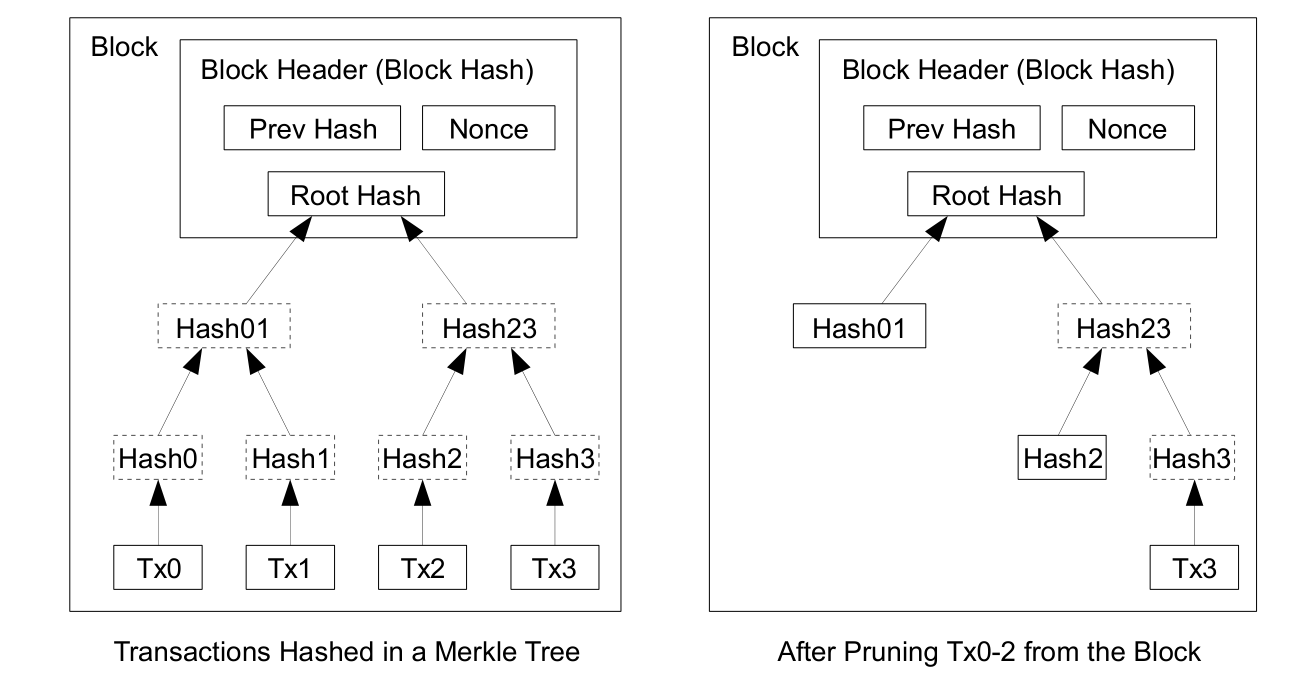
\includegraphics{bitcoin_p4_1.PNG}
\caption{Struttura di un blocco prima e dopo la compressione dell'albero delle transazioni.\label{bitcoin_p4_1}}
\end{figure}

%TODO sezione tecnica
Con questa struttura, il \textbf{block header} viene ad occupare esattamente 80 Bytes (vedi sezione tecnica per i dettagli), il che significa circa 6.2 MB all'anno (Satoshi Nakamoto con una stima di un blocco ogni 10 minuti aveva previsto 4.2 MB annui). Una quantità decisamente ridotta che rende la blockchain tollerabile su ogni computer degli ultimi 7 anni.

È possibile quindi verificare i pagamenti senza disporre di un nodo personale. L'utente deve possedere una copia degli header della catena più lunga (che può ottenere dai nodi della rete) e ottenere il ramo di Merkle che collega la transazione al blocco in cui è stata inserita. Non può verificare la transazione da solo calcolando gli hash (non ha le altre foglie dell'albero di Merkle), ma collegandola ad un punto specifico della catena può vedere che un nodo l'ha accettata, ed eventuali blocchi successivi confermano che anche l'intera rete l'ha accettata.

\begin{figure}[htbp]
\centering
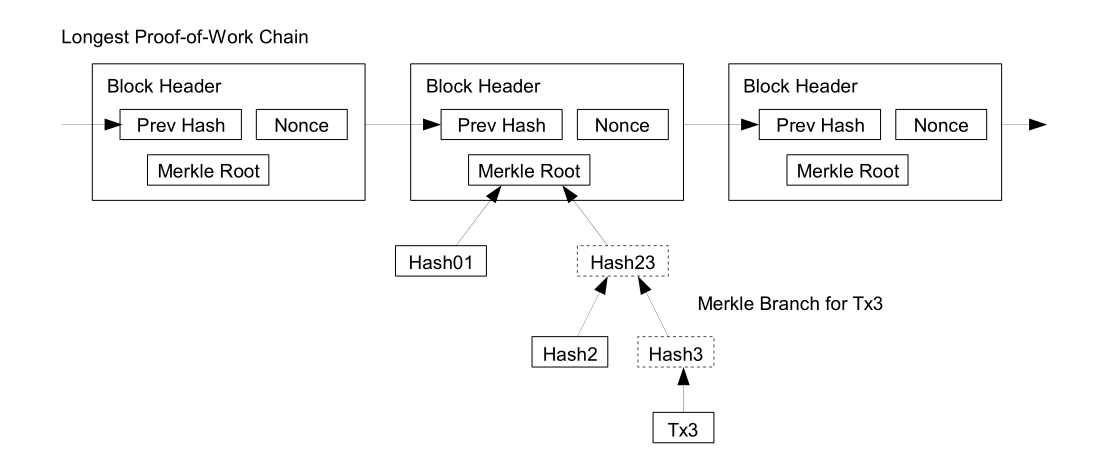
\includegraphics{bitcoin_p5_1.PNG}
\caption{Struttura di un blocco prima e dopo la compressione dell'albero delle transazioni.\label{bitcoin_p5_1}}
\end{figure}

Così come è descritta, la verifica è affidabile fin tanto che la rete è controllata da nodi onesti, ma è vulnerabile se la rete è soverchiata da un attaccante. Mentre un nodo può effettuare le verifiche da se, il metodo semplificato è vulnerabile alle transazioni ad-hoc create da un attaccante che controlla la rete. Una strategia di difesa consiste nell'accettare avvisi dai nodi della rete quando questi rilevano blocchi non validi, richiedendo all'utente di scaricare l'intero blocco. Per questo motivo chi utilizza bitcoin per business ritiene preferibile avere un nodo personale con intera blockchain, in modo da poter effettuare verifiche autonomamente e velocemente. 
%FIXME questo paragrafo è scritto male

Da questo si può dedurre un fatto importante che distingue la rete bitcoin dalle altre reti P2P: si può partecipare alla rete anche senza il relativo software (in questo senso, si partecipa al livello comunitario della rete): non serve essere un nodo, basta essere un utente.

\section{Gestione dei valori}\label{gestione-dei-valori}

Anche se è possibile trattare le monete una ad una, è improponibile fare una transazione per ogni singolo centesimo. Per la divisione degli importi, le transazioni contengono molteplici input e output. In una transazione normale si avranno o un singolo input proveniente da una grande transazione precedente oppure più input provenienti da più transazioni piccole precedenti, e al massimo due output: uno per il pagamento vero e proprio e uno per restituire il resto, se presente, al mittente.

Chiarimo meglio il concetto:

\begin{itemize}
\itemsep1pt\parskip0pt\parsep0pt
\item
  Un input è un riferimento ad un output di una precedente transazione   che contiene l'indirizzo di chi sta effettuando la transazione. Se ci   sono più input, l'importo degli output da loro referenziati viene   sommato ed il totale è il massimo valore utilizzabile dall'output.
\item
  Un output contiene l'indirizzo del destinatario e il valore da   spedire. Dato che, in una futura transazione, un output può essere   referenziato da un solo input, potrebbe verificarsi il caso in cui   l'input sia maggiore dell'output e della transaction fee desiderata.   In questo caso è necessario creare due output, uno con il valore da   spedire e l'indirizzo del destinatario, l'altro con la differenza da   restituire al mittente, il \textbf{resto}. La differenza tra il totale   degli input e il totale degli output è la transaction fee.
\end{itemize}

La situazione è visibile in \ref{bitcoinpropagation_1}.

\begin{figure}[htbp]
\centering
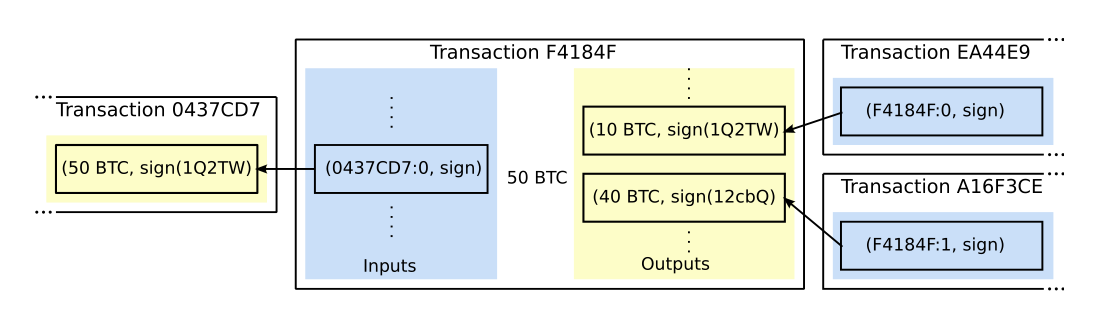
\includegraphics{bitcoinpropagation_1.PNG}
\caption{Schema di una transazione in cui vengono evidenziati input e output.\label{bitcoinpropagation_1}}
\end{figure}

Nonostante la stretta dipendenza tra le varie transazioni, non è necessario estrarre l'intero background di ogni input, in quanto la transazione verrà accettata solo se il blocco che contiene le transazioni con gli output referenziati dagli input è stato accettato dalla rete.

Dato il valore elevato di una singola btc (che può variare da poche decine a migliaia di dollari) e le difficoltà inerenti nel trattare numeri in virgola mobile su un computer, l'unità di misura base della transazione non è il btc ma il Satoshi \footnote{dal ``nome''   dell'inventore di Bitcoin}, e 1 BTC = 100000000 Satoshi.

Questo sistema del calcolo del valore di una transazione è lo stesso utilizzato dal software che gestisce il portafoglio per calcolare il proprio valore: per ogni indirizzo all'interno del portafogli, il software scansiona le transazioni presenti nella blockchain che contengono l'indirizzo in esame, somma i valori entranti nell'indirizzo, sottrae quelli uscenti e ricava il valore ``contenuto'' nell'indirizzo. Usando questo sistema, i possedimenti di un utente sono temporalmente limitati all'ultimo blocco accettato nella catena, e non è quindi possibile spendere moneta ricevuta da una transazione non ancora approvata \footnote{tecnicamente, nessuna moneta è ricevuta fin tanto   che la transazione non è approvata. L'utente non è nemmeno consapevole   della transazione a lui destinata fino ad avvenuta approvazione.}.

\%\%\%\%\%\%\%\%\% \% La documentazione di Satoshi prevede anche privacy e calcoli statistici sugli attacchi. \% Visto che prevedo una sezione apposta per anonimato e sicurezza, ne parlo la e non qua. \% Attenzione che la parte di topologia successiva nomina alcuni risultati statistici di questa parte\ldots{} una volta scritta saranno da fare i collegamenti

\section{Analisi della rete}\label{analisi-della-rete}

Sappiamo che i nodi della rete Bitcoin sono tutti omogenei e nessuno di essi ha un ruolo di coordinatore o comunque diverso da quello degli altri nodi, e ognuno di essi mantiene una copia di tutte le informazioni necessarie per far funzionare il sistema. Vediamo ora più formalmente come si struttura la rete Bitcoin e come le informazioni (ovvero, le transazioni e i blocchi) si propagano in essa.

\subsection{Topologia}\label{topologia}

Non essendoci coordinazione tra i nodi, il grafo rappresentante la rete ha una struttura casuale. Durante il \emph{churm} il nuovo nodo interroga alcuni server DNS gestiti da nodi volontari e si vede restituiti un insieme casuale di nodi con cui fare il bootstrap. Una volta connesso, impara dai suoi vicini gli indirizzi dei nodi raggiungibili e si mette in ascolto nel caso nuovi nodi vengano annunciati in broadcast. A differenza di una rete P2P ``tradizionale'', non esiste alcun modo per un nodo di lasciare la rete: gli indirizzi restano memorizzati per diverse ora prima che gli altri nodi li rimuovano dalla loro lista di indirizzi noti.

Ogni nodo tenta di mantenere un certo numero \emph{p} di connessioni con gli altri nodi, collegandosi ad un indirizzo scelto a caso tra quelli che conosce nel caso il numero di connessioni sia inferiore a \emph{p} ma senza bloccare connessioni in ingresso nel caso tale sumero sia superiore. Il valore \emph{p} rappresenta quindi un valore minimo di connessioni spesso e volentieri superato per nodi abilitati ad accettare connessioni in ingresso. Per il client \emph{bitcoind}, il primo implementato da Nakamoto e tutt'ora il più diffuso, il default è $p=8$, ma il numero medio di connessioni contemporanee è 32 nel caso in cui non ci siano firewall o NAT \footnote{Network Address Translator: maschera   gli indirizzi di una LAN come un unico indirizzo IP sulla rete   Internet, e spesso impedisce a host presenti in Internet di   connettersi ad host specifici in una LAN.} ad intercettare connessioni esterne.

%TODO sistemare paragrafo seguente 
Dato il tipo di connessione tra i nodi, le partizioni non sono individuabili nel momento in cui si creano e, nel caso in cui dovessero esistere, esse continuerebbero ad operare indipendentemente. Una tale situazione comporta nel tempo una divergenza tra le situazioni tracciate dalle due partizioni, situazioni potenzialmente incompatibili. Pertanto è fondamentale individuare le partizioni nel momento in cui si creano, e uno dei modi per farlo è tracciare il potere computazionale complessivamente presente nella rete: una rapida diminuzione della frequenza di creazione di blocchi può indicare la presenza di una partizione.

\subsection{Propagazione delle informazioni}\label{propagazione-delle-informazioni}

Per ciò che riguarda il mantenimento della blockchain, solamente i messaggi di transazione \emph{tx} e i blocchi sono rilevanti. Tali messaggi sono molto più comuni di tutti gli altri scambiati nella rete e potrebbero raggiungere dimensioni rilevanti. Per evitare di sprecare banda e ridurre l'overhead, è necessario fare in modo di inviare ognuno di questi messaggi una sola volta per ogni nodo, evitando quindi l'inoltro ai nodi che già hanno ricevuto quel messaggio.

L'implementazione utilizzata da Bitcoin sfrutta una tecnica passiva: invece che inoltrare tutti i messaggi, ogni nodo dopo aver verificato un messaggio o una transazione invia a suoi vicini un messaggio \emph{inv} per segnalare la disponibilità di nuovi tx o blocchi. Il messaggio \emph{inv} contiene gli hash dei blocchi e delle transazioni disponibili per l'invio, che ogni vicino può richiedere nel caso gli mancasse tramite un messaggio \emph{getdata}. I messaggi \emph{inv} e \emph{getdata} (61 B) sono ovviamente significativamente più piccoli dei messaggi \emph{tx} e \emph{block} (fino a 500 kB per i blocchi).

Ogni volta che si verifica lo scambio di \emph{inv} e \emph{getdata}, la velocità di propagazione del messaggio subisce un rallentamento, dovuta sia allo scambio di messaggi sia alla necessità di verificare la transazione/blocco con calcoli crittografici: bisogna verificare ogni nodo prima di notificarne la disponibilità, e tale verifica include la verifica di ogni transazione nel blocco, le quali a loro volta richiedono accesso random ai dati del disco rigido.

Vediamo di stimare formalmente come si propaga un dato nella rete.

Definiamo $t_{i,j}$ come il tempo trascorso tra il primo annuncio e il momento in cui il nodo $j$ riceve l'oggetto $i$. Il nodo $o$ sarà l'origine dell'oggetto $i$ (ovvero il nodo che ha trovato il blocco o il nodo che ha creato la transazione), quindi $t_{i,o}=0$.

%TODO tradurre ``double exponential''
Il tempo $t_{i,j}$ ha un comportamento \textbf{doppio esponenziale}. Il periodo di propagazione segue due fasi: una prima crescita esponenziale in cui la maggior parte dei nodi che ricevono un \emph{inv} richiederanno il relativo dato che non possiedono, e una seconda fase di compressione esponenziale in cui la maggior parte dei nodi che ricevono un \emph{inv} hanno già il dato.

Per effettuare le loro misurazioni, i ricercatori Christian Decker e Roger Wattenhofer dello Swiss Federal Institute of Technology di Zurigo hanno implementato il protocollo bitcoin su un nodo creato in modo tale da non inviare messaggi \emph{inv}, \emph{tx} o \emph{block} e collegato a direttamente a quanti più nodi tradizionali possibile. Tale implementazione ha il solo scopo di tracciare come i blocchi si propagano nella rete restando in ascolto dei messaggi \emph{inv} che ne annunciano la disponibilità \cite{bitcoinpropagation}. La ricezione di un \emph{inv} implica che il nodo che ha inviato il messaggio ha ricevuto e verificato un blocco.

La rilevazione è partita su nodi di altezza 180000 ed è durata per 10000 blocchi. Le informazioni rilevate includono l'hash del blocco, l'IP del noto annunciante e una timestamp della ricezione dell'\emph{inv}. La stima per $t_{i,j}$ è ottenuta sottraendo il timestamp del primo annuncio di un blocco da tutti gli annunci successivi per quel blocco. I risultati sono riassunti nel grafico \ref{bitcoinpropagation_3}.

\begin{figure}[htbp]
\centering
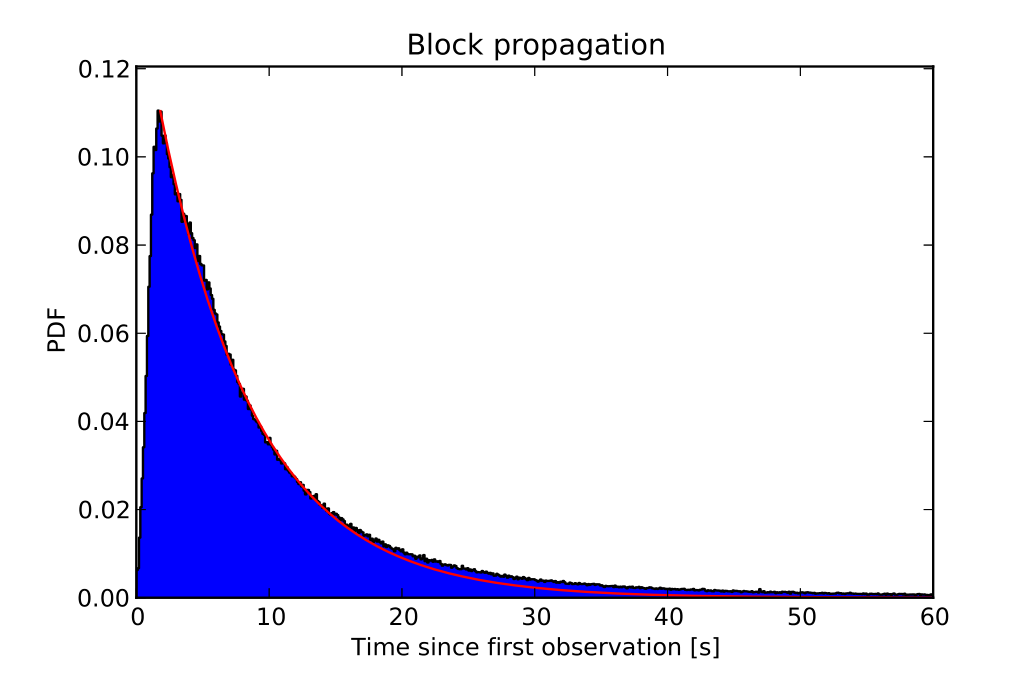
\includegraphics{bitcoinpropagation_3.PNG}
\caption{Istogramma normalizzato del tempo che intercorre dal primo annuncio del blocco con una curva di interpolazione esponenziale.\label{bitcoinpropagation_3}}
\end{figure}

Le misurazioni effettuate ci permettono di stabilire che il tempo mediano in cui un nodo riceve un blocco è di 6.5 secondi, mentre la media è di 12.6 secondi. La lunghezza della seconda fase, quella di contrazione esponenziale, evidenzia come dopo soli 40 secondi il 95\% dei nodi abbia ricevuto il blocco.

Abbiamo però detto come la dimensione di un blocco sia variabile, fino a 500kB. I dati precedenti sono aggregati per tutti i blocchi e non tengono conto delle differenti dimensioni degli stessi. Perciò definiamo ora il \emph{costo di ritardo} come il ritardo che ogni kB causa alla diffusione di una transazione o di un blocco. Tale costo risulta essere una combinazione sia del tempo di trasmissione che del tempo di verifica. I risultati sono contenuti nel grafico \ref{bitcoinpropagation_4}.

\begin{figure}[htbp]
\centering
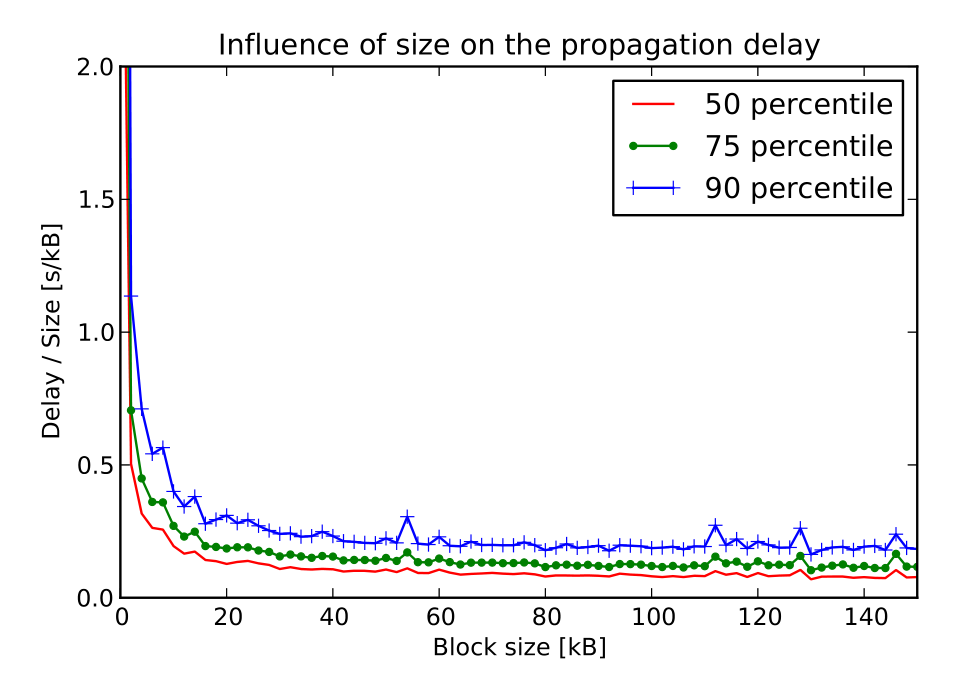
\includegraphics{bitcoinpropagation_4.PNG}
\caption{Costo del ritardo per il 50°, 75° e 90° percentile. Il grafico è focalizzato sui valori più bassi delle ascisse per poter mostrare il comportamento costante presente dopo i 20kB.\label{bitcoinpropagation_4}}
\end{figure}

%TODO tradurre roundtrip delay
Per pacchetti di dimensione superiore ai 20kB si vede come il costo sia pressoché costante, mentre per dimensioni minori si assiste a notevole ritardo. La causa di ciò sta nel \textbf{ritardo da un roundtrip}, ovvero il fatto che anche i piccoli messaggi vengono annunciati con \emph{inv} e richiesti con \emph{getdata}. Il roundtrip è dominante per le transazione in quanto il 96\% di tutte le transazioni sono inferiori ad 1kB. Per i blocchi, la cui dimensione è per la maggior parte superiore ai 20kB, ogni kB di dimensione costa circa 80ms di ritardo fino al momento in cui la maggioranza dei nodi non ha il blocco. %TODO verificare questa frase, sembra l'esatto opposto di quanto scritto nel grafico
Nel caso di piccoli blocchi sarebbe pertanto ottimale evitare l'annuncio e inoltrare direttamente il blocco ai nodi vicini.

\subsection{Informazioni scomparse}\label{informazioni-scomparse}

Trattiamo ora il caso in cui un blocco inoltrato in rete porti ad un fork della blockchain che viene rilevato solo da una piccola parte dei nodi.

Definiamo il grafo che descrive la rete come $G = (V,E)$, con $V$ i nodi (vertici) ed $E$ le connessioni tra i nodi (archi/edges). Definiamo inoltre la partizione $P_h \subset V$ come l'insieme dei nodi il cui blocco di testa si trova ad altezza $h$. Trovare un nuovo nodo $b_{h+1}$ crea una nuova partizione $P_{h+1,b}$ contenente i nodi che considerano questo nuovo blocco come blocco di testa, in altre parole questo è il primo blocco di altezza $h+1$ che abbiano ricevuto. Se non vengono trovati altri blocchi, allora i nodi di $P_h$ adiacenti a $P_{h+1,b}$ si uniscono a $P_{h+1,b}$ lasciando (e quindi eliminando) la partizione $P_h$. Dal'altro canto, se viene trovato un blocco $b'_{h+1}$ da un nodo in $P_h$ viene creata una nuova partizione $P_{h+1,b'}$. Anche in questo caso i nodi di $P_h$ abbandoneranno la loro partizione per unirsi ad una delle due nuove di altezza superiore. Solamente i nodi di $P_h$ che sono a contatto sia con $P_{h+1,b}$ che con $P_{h+1,b'}$ saranno consapevoli dell'esistenza di entrambe le partizioni e quindi del fork della blockchain, e considereranno invalido il blocco di altezza $h+1$ proveniente dall'altra partizione e di conseguenza non lo annunceranno ai loro vicini fermando quindi l'espansione della partizione. Tale meccanismo si applica anche alle transazioni: se due tx tentano di spendere lo stesso output, solo la prima transazione ricevuta da un nodo verrà considerata valida, la seconda verrà considerata invalida e non annunciata ai vicini. Questo comportamento ha il vantaggio di impedire ad un nodo malevolo di inondare la rete con centinaia di transazioni contraddittorie senza costo addizionale, in termini di transaction fees, per il nodo malevolo. Il rovescio della medaglia è che questo sistema di nascondere le informazioni ritenute sbagliate da un nodo permettere l'implementazione di \textbf{attacchi double spend} che risultano invisibili ai commercianti. Nel caso delle transazioni, dato che esse non devono per forza propagarsi a tutti i nodi, il meccanismo descritto è ragionevole e protegge la rete da transazioni spam. Nel caso dei blocchi invece, fermarne la propagazione è controproducente: i fork della blockchain, che con tale sistema sono invisibili per la maggior parte dei nodi, sono una cartina tornasole che indica come nella rete ci siano alcune inconsistenze non risolte. Dato che i blocchi valido ma potenzialmente in conflitto non possono essere creati con un frequenza arbitraria come le transazioni, permettere il loro inoltro anche nel caso di conflitto non crea possibilità per un potenziale attacco.

\section{Fork della blockchain}\label{fork-della-blockchain}

Durante il normale utilizzo della rete potrebbe capitare di essere testimoni di un fork se si ricevono due blocchi conflittuali, ma osservare tutti fork che avvengono è molto difficile a causa della non propagazione dei blocchi in conflitto discussa in precedenza. Se a questo aggiungiamo il fatto che una partizione potrebbe avere dimensione unitaria (un nodo genera un nuovo blocco in conflitto con il blocco di testa di tutti i suoi vicini) è evidente come per poter rilevare tutti i fork bisognerebbe connettersi ad ogni nodo della rete. Ma abbiamo detto che alcuni nodi non sono raggiungibili dall'esterno, per cui possiamo solo stimare il numero di fork che avvengono.

Utilizzando la configurazione descritta nella sezione precedente, sono stati raccolti tutti i blocchi di altezza compresa tra 180000 e 190000. Essendo un grande campione che coinvolge tutti i nodi raggiungibili, è abbastanza probabile che tutti i blocchi generati siano stati propagati fino al nodo spia implementato permettendo di individuare la maggior parte dei fork avvenuti nell'intervallo di rilevazione. Nei 10000 blocchi osservati sono stati identificati 169 fork, il che si traduce in rateo di forking $r = 1.69\%$. L'istogramma \ref{bitcoinpropagation_5} mostra i risultati in modo più dettagliato.

\begin{figure}[htbp]
\centering
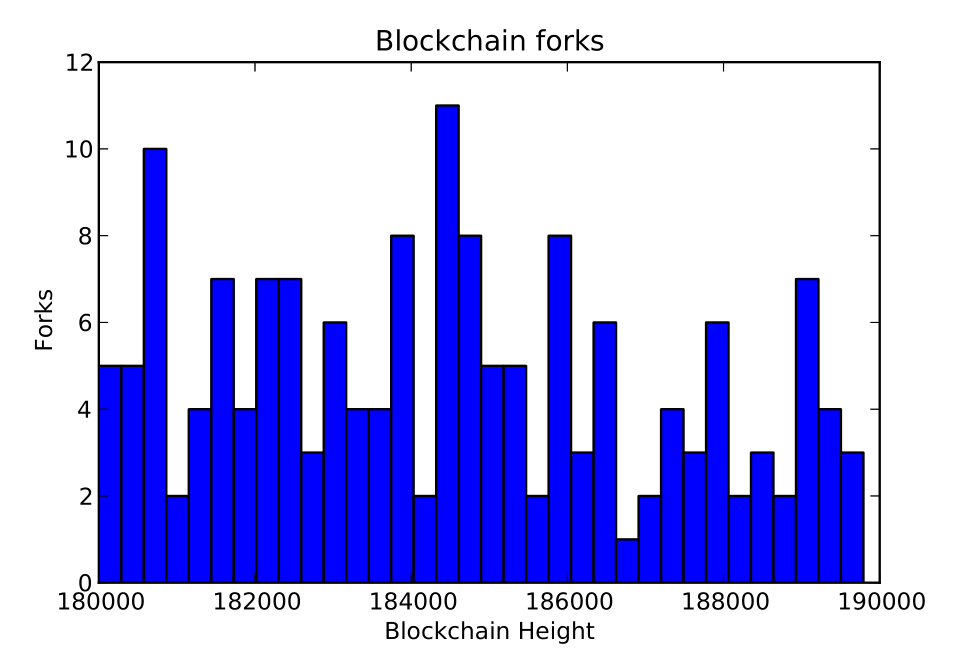
\includegraphics{bitcoinpropagation_5.PNG}
\caption{Fork osservati tra i blocchi 180000 e 190000 durante il collegamento alla rete.\label{bitcoinpropagation_5}}
\end{figure}

\subsection{Creazione del modello}\label{creazione-del-modello}

Il protocollo bitcoin adatta la difficoltà della proof-of-work ogni 10 minuti in modo da mantenerla sufficientemente elevata da essere significativa. Definendo $X_b$ come la variabile casuale che rappresenta i secondi trascorsi tra il ritrovamento di un nodo e il ritrovamento del nodo precedente, allora la \emph{probabilità che un blocco venga trovato} nella rete in un dato secondo è

\[ P_b = \Pr\left[ X_b < t + 1 | X_b \geq t\right] \approx 1/600 \]

Un fork avviene se, durante la propagazione del blocco $b$, viene trovato un blocco $b'$ in conflitto nella parte di rete non ancora a conoscenza di $b$. Definiamo $t_j$ come il tempo in secondi in cui $j$ apprende dell'esistenta di $b$ da quando esso è stato creato. La funzione $I_{j}(t)$ identifica se il nodo $j$ sa dell'esistenza di $b$ nell'istante $b$, e la funzione $I(t)$ conta il numero di nodi che hanno ricevuto e verificato $b$ all'istante $t$.

\[ I_{j}(t) = \begin{cases}
    0 &\textrm{se } t_j > t \\
    1 &\textrm{se } t_j \leq t
\end{cases}\]

\[ I(t) = \sum_{j \in V} I_{j}(t) \quad  \textrm{con }V\textrm{ insieme dei vettori} \]

Da cui ottengo il rateo di nodi informati:

\[ f(t) = \mathbb{E}[I(t)] \cdot n^{-1} \]

Notare come la $f(t)$ sia equivalente alla funzione di distribuzione cumulativa (\textbf{CDF}) della frequenza alla quale i peer vengono informati. Possiamo quindi utilizzare la funzione di densità di probabilità (\textbf{PDF}) della frequenza con cui i peer vengono informati rappresentata in \ref{bitcoinpropagation_3} come una approssimazione durante le rilevazioni. Solo i nodi non informati possono produrre blocchi in conflitto, per cui combinando la probabilità di trovare un blocco con il rateo di nodi non informati otteniamo la probabilità di un fork. Definiamo $F$ come la variabile casuale discreta che conta il numero di blocchi in conflitto trovati mentre un altro blocco viene propagato. Allora la propabilità di un fork risulta:

\[ \Pr\left[F \geq 1\right] = 1 - (1 - P_b)^{\int_{0}^{\infty} \! (1 - f(t)) \, \mathrm{d}t} \]

In questo ultimo passaggio si è assunta la semplificazione per la quale la probabilità di un nodo di trovare un blocco è distribuita uniformemente in modo casuale tra tutti i nodi.

Per cui, sapendo la probabilità dell'intera rete di trovare un blocco $P_b$ e la distribuzione di come i nodi apprendono dell'esistenza del blocco $I_j$, si può derivare la probabilità di un fork. Questi due valori dipendono dal potere computazionale della rete nonché dalla sua topologia e dimensione.

\subsection{Misurazioni}\label{misurazioni}

Per confermare il corretto funzionamento del modello proposto è necessario confrontare la probabilità ottenuta con i dati rilevati.

Bisogna innanzitutto notare come i nodi non sincronizzino i loro orologi interni, bensì si regolano sui loro vicini, esiste una differenza non trascurabile tra i timestamp. Ad esempio il blocco ad altezza 209873 ha un timestamp pari a 22:10:13 mentre il blocco ad altezza 209874 ha un timestamp di 22:08:44. Dato che il secondo include l'hash del primo, i blocchi sono stati trovati nell'ordine corretto. Da questo si deduce che il conflitto nei timestamp è derivato dalla mancata sincronizzazione degli orologi dei nodi.

%TODO il paragrafo seguente è scritto da cani.
%TODO scrivere che roba è un Processo di Poisson
In questa analisi si potrebbe tenere conto dell'orario in cui il nodo spia rileva l'annuncio del blocco e l'orario in cui il blocco è stato trovato. Anche se questo metodo non subisce la differenza di orario tra i nodi, potrebbe esistere un lieve ritardo tra il calcolo del blocco e la rilevazione del relativo annuncio, e per la misurazione abbiamo a disposizione solo il timestamp del blocco. Dato che il calcolo della proof-of-work è un processo di Poisson, la differenza temporale segue una distribuzione esponenziale. La combinazione della differenza temporale degli orologi e il tempo intercorso tra i ritrovamenti dei blocchi causa uno spostamento a destra del massimo. Possiamo correggere la situazione spostando a sinistra fin quando il massimo non risulta in $t=0$. L'orario di annuncio rilevato durante la misura non è influenzato dalla differenza temporale e produce l'istogramma corretto.

%TODO diagramma 6 pag 7 bitcoinpropagation

\[ g(t) = \lambda e^{-\lambda \cdot x}\]

Estraendo i timestamp dai blocchi tra altezza 180000 e 190000 si ottiene la distribuzione illustrata nel grafico \ref{bitcoinpropagation_6}. Interpolando la distribuzione ottenuta con la distribuzione esponenziale si ottiene $\lambda = 0.001578$ da cui risulta un tempo atteso tra due blocchi pari a $1 / \lambda = 633.68$ secondi. Interpolando la densità di probabilità del tempo tra i primi annunci e le misurazioni si ottiene $\lambda = 0.001576$ che si traduce in un tempo atteso tra due blocchi $1/ \lambda = 634.17$ secondi. Le due approssimazioni sono coerenti ma sono entrambe leggermente sopra il valore obiettivo di 600 secondi. La differenza è probabilmente dovuta ad un decremento del potere computazione della rete.

Per quando riguarda la propagazione dei nodi nella rete, a causa della normalizzazione il diagramma \ref{bitcoinpropagation_3} rappresenta anche la funzione di densità di probabilità (\textbf{PDF}) delle variabili casuali $t_{b,j}$ per tutti i blocchi $b$ dell'intervallo di misurazione. Per cui la frequenza dei nodi informati $f(t)$ è l'area che sottostà all'istogramma \ref{bitcoinpropagation_3} fino al tempo $t$.

\begin{figure}[htbp]
\centering
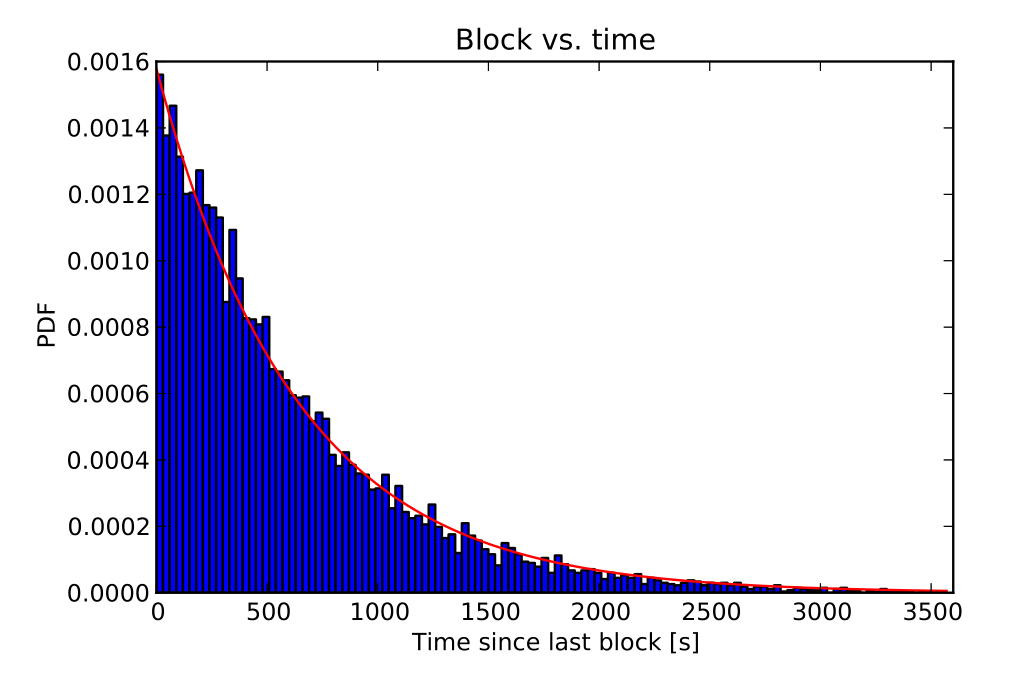
\includegraphics{bitcoinpropagation_6.PNG}
\caption{Tempo di distribuzione spostato a sinistra per i blocchi trovati tra le altezze 180000 e 190000.\label{bitcoinpropagation_6}}
\end{figure}

Combinando la probabilità di trovare un blocco e la funzione della frequenza dei nodi informati si ottiene la seguente probabilità per un fork:

\begin{equation}
\begin{aligned}
    \Pr [F \geq 1 ] &= 1 - (1 - P_b)^{\int_{0}^{\infty} \! (1 - f(t)) \, \mathrm{d}t} \\
    &= 1 - (1 - \frac{1}{633.68})^{11.37} \\
    &\approx 1.78%
\end{aligned}
\end{equation}

Comparando questo risultato con quello osservato di 1.69\% si nota di aver sovrastimato il valore osservato solo del 5\%. Il risultato leggermente superiore può essere spiegato dall'assunto fatto che la potenza di calcolo sia uniformemente distribuita tra tutti i nodi nella rete. Ciononostante, il buon risultato ottenuto dimostra come il modello sia una efficace rappresentazione della realtà.

Dato che il numero di transazioni e le dimensioni della rete molto probabilmente cresceranno mano a mano che aumenta l'adozione di Bitcoin, la frequenza dei fork è destinata a salire. Una rete più grande, con una topologia casuale e il numero di connessioni limitate per singolo nodo, aumenta il suo diametro e la distanza media tra i nodi e l'origine di un blocco. L'aumento del numero di transazioni provoca una crescita nella dimensione dei blocchi il che a sua volta aumenta il tempo necessario per la verifica e la trasmissione ad ogni passo della propagazione.

%TODO da qui in poi sono problematiche al metodo di propagazione. Sarebbe il caso di metterlo nel capitolo problemi e soluzioni

Una interpretazione alternativa del risultato proposto in %TODO link all'equazione precedente
è che ogni volta che un blocco viene trovato, l'equivalente di 11.37 secondi di potere computazionale dell'intera rete viene sprecato. Infatti il lavoro impiegato per trovare il primo blocco di una blockchain alternativa (che potrebbe essere scartata) non contribuisce alla sicurezza della rete e costituisce un eventuale punto a favore di un attaccante che cerca di implementare una sua blockchain alternativa. Come detto in precedenza da Nakamoto, un attaccante capace di controllare più del 50\% del potere computazione delle rete è in grado di trovare proof-of-work più velocemente di tutto il resto il della rete. L'attaccante sarebbe perciò in grado di rimpiazzare l'intera storia delle transazione a partire da un qualsiasi blocco. Pur sicuramente sufficiente, questa condizione non è minima. In realtà l'efficenza della rete come intero, incluso il ritardo di propagazione, non è ottimale. La potenza computazionale effettiva nella rete così come si presenta a Settembre 2013 è pari a $1 - 11.37 / 633.68 = 98.20\%$. Per cui ad un attaccante basta controllare il 49.1\% della forza di calcolo della rete per poter portare un attacco e cambiare la blockchain. Al momento questo è un risultato difficile da ottenere, ma la situazione potrebbe cambiare in peggio a causa dell'aumento costante del ritardo di propagazione.
